% !TEX root = ../Thesis.tex

%beschrijving van het opgeleverde eindproduct, plusminus 15 pagina’s
\section{Design \& Implementation}
\label{sec:design-implementation} 
In this section, we depict the high-level architecture of the new parser.
We do this by first giving an architecture overview in \autoref{design:system-overview}.
Then we elaborate on the code quality in \autoref{design:software-quality}.
The new lexer is described in \autoref{design:new-lexer}, while the parser itself is presented in \autoref{design:new-parser}.
The new test suite and the improved error messages are described later in \autoref{sec:tests}.
Additionally, more detailed artifacts are given in the \hyperref[app:docs]{project documentation (appendix)}.

% !TEX root = ../Documentation.tex

\subsection{System overview (R-M)}
  The parser module overview is given in \autoref{fig:ParserModules}.
  \begin{figure}[ht]%
    \centering
    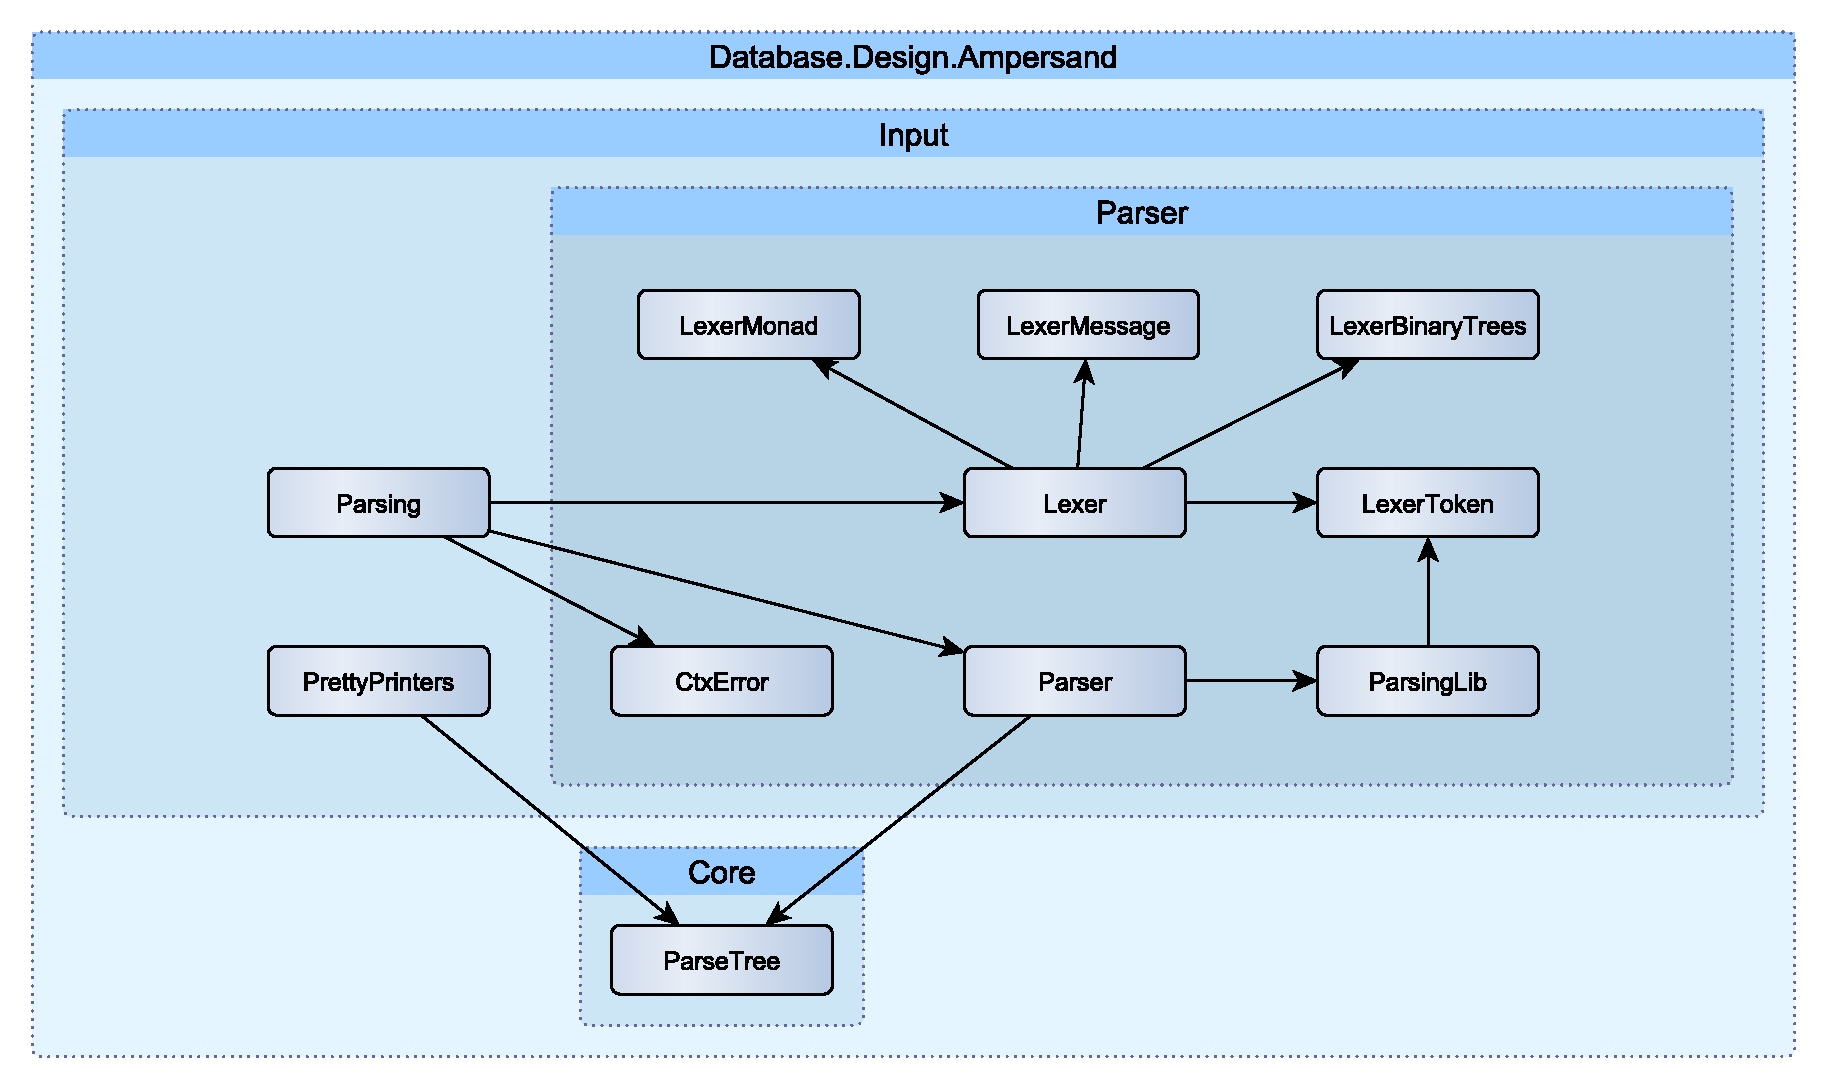
\includegraphics[width=0.7\columnwidth]{Figures/ParserModules}
    \caption{The modules relevant for the parser and their relationships}
    \label{fig:ParserModules}
  \end{figure}%
  Each module has the following responsibilities:
  %
  \begin{description}
    \item[Parsing] module that implements the interface of the parser with the rest of the system.
      It is responsible for reading the input files, calling the lexer and the parser and returning a parse tree as result (or a parse error).

    \item[Parser] module responsible for executing the parsing itself.
      It accepts the tokens that are allowed in each grammar production and generates the corresponding parse tree.
      The parser is described in \autoref{design:new-parser}.
      
    \item[ParsingLib] library that contains several useful functions to assist the parser, e.g. token recognition.
      These functions are not depending on the specific grammar rules.
      
    \item[ParseTree] external module containing the parse tree data structures.
      Only details of this module have been changed during this project (e.g. field ordering).
    
    \item[PrettyPrinters] contains the \texttt{Pretty} class and the functions responsible for printing the parse tree to ADL scripts in a `pretty' way.
    
    \item[CtxError] contains the data structures responsible for the parse errors and their location.
      This module has not been refactored as a part of this project.
    
    \item[Lexer/LexerToken] modules responsible for recognizing the input characters and converting them to tokens.
      The new lexer, together with its sub-modules, is described in \autoref{design:new-lexer}.
  \end{description}

% !TEX root = ../Thesis.tex

\subsection{Software quality factors}
\label{design:software-quality}
In our project plan \citepr{plan} multiple non-functional requirements are included in the project scope.
Improving the code maintainability is one of the most important non-functional requirements.

To assure that these non-functional requirements are correctly addressed, we defined some measures to adhere to during the full project life cycle.

\subsubsection{Documentation}
All important design decisions we made together with the code we delivered need to be documented.
This documentation is needed for the Ampersand team to have a clear insight in the way the new parser is structured and how it is integrated in Ampersand.
The availability of this documentation is crucial for the maintainability of the new parser.
The following documentation is delivered as a result of this ABI project:
%
\begin{description}
  \item[System design]
    A general system overview of the new system, describing the goal and purpose of each module, how it is designed to achieve its goals and how it is integrated in the system architecture.
   The system design is integarted in this thesis document.
  \item[Code annotations]
    Haddock is the de-facto standard for generating Haskell documentation. 
    This documentation generator generates HTML based on the comments in the Haskell source code.
    It is important to remark that Haddock normally only generates documentation of the functions that are exported by each module.
    It is however important that all functions are well documented, including the internal ones, and therefore, the internal functions are documented using regular, non-Haddock, code annotations.
    The code annotations, in the source code, together with the Haddock documentation are delivered as an appendix to this document.
  \item[EBNF comments]
    The EBNF structure is the most important documentation of how the Ampersand syntax is composed and how the parser functions are defined.
    As described in \autoref{analysis:grammar}, the actual EBNF is retrieved through reverse engineering.
    Each parser function corresponds to a specific EBNF syntax rule and this rule is consistently annotated in the code just above the parse function.
  A specific markup (\code{------}) is used to tag the EBNF rules.
  This allows us to automatically extract the EBNF rules from source code and export them to other formats.
\end{description}

\subsubsection{Readability}
  In the as-is analysis of the current parser, we noticed that the code has been through several feature additions over the past years.
  These repetitive small changes reflected in parts of the code which has become too elaborated or sometimes even obsolete.

  Each code statement in the parser and lexer is analyzed by the project team and, where possible, refactored to be as concise as possible.
  The delivered code is now as short as possible without compromising the readability of the code.

  In addition, the code review tool HLint is used.
  This tool provides a full overview of several code optimization suggestions that can further optimize the readability of the source code. 
  These suggestions cover topics such as redundant brackets, parameter reductions and shortcut notations.
  All HLint warnings regarding the input subsystem are fully addressed before the code is delivered to the customer.
  The HLint report for the delivered code is available in the \hyperref[app:docs]{project documentation (appendix)}.

\subsubsection{Performance}
  Performance is a requirement often made in software engineering projects that is difficult to measure before the software is actually used in a production environment.
  For the new Ampersand parser, we proactively identified the topics that could have an impact on the resulting parsing performance.
  In the design of the new parser, a performance aspect that makes an important difference is the parser backtracking (with the \code{try} function).
  Several refactorings in the grammar are carried through to avoid the use of the \code{try} function. 
  A full list of remaining backtracking productions, together with our suggestions how to solve them, is provided in section \autoref{design:backtracking}.

% !TEX root = ../Thesis.tex

\subsection{New Lexer}
\label{design:new-lexer}

\subsubsection{The rationale behind the new lexer}
In the design of the new Ampersand parser, the first decision to tackle is whether to keep the existing scanner/lexer or to implement a new one.
In the analysis of the error improvement areas in \autoref{sec:analysis}, the main improvements are identified within the old parser.
The error feedback quality, produced by the scanner module, is higher and therefore, there is no stringent need to re-implement the scanner.
On the other hand, given the aspect that Parsec is identified as the new parser library, keeping the current scanner would result in the utilization of two different libraries providing more of less the same functionality.

The alternative of keeping the existing scanner would deliver a perfect functional solution, but mixing these two libraries would increase the complexity of the solution, thus decreasing the maintainability.
To avoid this decrease in maintainability, the decision is to implement the parser and scanner based on the same library.

During the implementation of the lexer module, replacing the old scanner, additional attention was given to further improve the quality of the error messages.
The scanner module is renamed to lexer to stress the aspect that the principle of lexemes is used in the new scanner.
Lexemes can be seen as the part of a token containing the actual language content besides the actual position information.

The lexer is built based on the existing Helium lexer modules. 
Helium is a Haskell compiler with the main goal of giving user friendly error messages \citeac{helium}.
The lexer module in Helium contains interesting principles such as position monitoring, warnings and easy maintainable error messages.

% !TEX root = ../Documentation.tex

\subsubsection{Lexer structure}
The lexer is the main module, in which the actual lexing is done, and to do so, it uses the following sub-modules:

 \begin{description}
 
    \item[LexerMonad] contains a monad definition that supports lexing with context.
      It tracks for example the location in the input and the warnings that may be generated.
      This module is based on the Helium lexer, without any modifications to the used functions.
      All unused functions are removed to improve the code maintainability.
      
      The following functions or types are used in the Ampersand lexer:
	  \begin{itemize}
		\item \textbf{LexerMonad} is the main monadic type used in the lexer returning an error or a list of tokens together with a list of warnings
		\item \textbf{addPos} is used to trace the position of the token
		\item \textbf{lexerError} to generate lexer error
		\item \textbf{lexerWarning} to generate lexer warnings
		\item \textbf{runLexerMonad} main function to handle the \code{LexerMonad} results 
	  \end{itemize}
	  
    \item[LexerMessage] contains functions to handle errors and warnings from the lexer.
	  Based on the warning/error type and the needed language, \code{LexerMessage} will fetch the correct description of an error or a warning out of the \code{LexerTexts} module.
	  The show functions for the error and warning are maintained in this module.
	  
    \item[LexerTexts] fetches the correct description of an error or a warning out of the \code{LexerTexts} module.
	  The centralization of the error message texts provides an easy entry point for the maintenance of the actual messages as these messages are no longer dispersed over the module functions.
	  
    \item[LexerBinaryTrees] module responsible for searching binary trees in an efficient way, to support the token recognition.
    This is the previously existing \code{UU\_BinaryTrees} module which is renamed to match the used naming structure of the new lexer modules.

    \item[LexerToken] contains the data structure and corresponding show function that represents the input tokens for the lexer.
	
  \end{description}


\subsubsection{New token structure}
Based on the improvement topics mentioned in \autoref{analysis:lexer}, a new token structure is defined.
Each token contains the lexeme: a part of the input string defining the token type and content, plus the position of the token in the input file.
The token structure is defined as follows:

\begin{haskell}
data Token = Tok { tokLex :: Lexeme    -- ^ The lexeme (defined below)
                 , tokPos :: FilePos   -- ^ The file position
                 }

data Lexeme  = LexSymbol      Char     -- ^ Single character
             | LexOperator    String   -- ^ Operator
             | LexKeyword     String   -- ^ Keyword
             | LexString      String   -- ^ String
             | LexExpl        String   -- ^ Explanation
             | LexAtom        String   -- ^ Atom
             | LexDecimal     Int      -- ^ Decimal integer
             | LexOctal       Int      -- ^ Octal integer
             | LexHex         Int      -- ^ Hexadecimal integer
             | LexConId       String   -- ^ Upper case identifier
             | LexVarId       String   -- ^ Lower case identifier
  deriving (Eq, Ord)
\end{haskell}
%
\code{Lexeme} is the combination of the token type and the actual token content, sliced from the input string.
\code{FilePos} is used to keep track of the original position of the lexeme in the input string.

During the lexer processing, the input file is processed sequentially.
All kinds of different accepted constructions are checked in a specific order.
Each time a match is found, the lexeme is extracted from the input string and a token is created.
In the token creation (function \code{returnToken}), the position and the lexeme are grouped into a token, then the next lexer iteration is started.

% !TEX root = ../Thesis.tex

\subsection{New Parser (R-M)}
\label{design:new-parser}
The mainstream design of the new parser has not changed much.
While the new parser may still be recognizable for the Ampersand developers, several improvements have been made.

As decided during the research for domain \& techniques (see \autoref{domain:parsing}), the parser has been rebuilt with the Parsec combinator library.
Basically, each EBNF rule receives its own parser function.
Thanks to the combinator operators, each parsing function also looks very similar to its corresponding EBNF.

The applicative interface is consistently used.
By changing details of the implementation, e.g. the order of the fields in the parse tree, we have made many of the `rebuild' functions unnecessary.
For some parsers the amount of changes necessary in order to remove supporting functions was too large or even impossible with the current parse tree.

Note that in parts of the parser, the function syntax has substituted the record syntax for creating data objects.
This was done only when the code readability could be improved by doing so.

\subsubsection{Parsec}
\label{design:parsing-lib}
As mentioned earlier, and described in research context document \citenac{parsing}, the new Ampersand parser has been rebuilt with another parsing library, namely Parsec.
However, for the Ampersand developers, the source code of the parser will still look very familiar, thanks to the applicative interface.
For developers, the main differences between Parsec and the uulib are:
\begin{itemize}
  \item Parsec does not backtrack by default.
    In order to enable backtracking, the \texttt{try} function must be used.
    This is described in \autoref{design:backtracking}.
  \item Parsec does not try to solve parsing errors.
    The parser stops immediately after the first issue.
   This way, the user is not overwhelmed with irrelevant information.
    See also the error analysis in \autoref{design:errors}.
  \item Error messages are customizable by using the \texttt{<?>} operator.
    This is also suggested in \autoref{design:next-steps}.
  \item Some combinators have a different name, e.g. one must use \texttt{option} instead of \texttt{opt}.
    Assuming the documentation found on Hackage is clear and sufficient, interface differences are not documented here.
\end{itemize}

\subsubsection{Backtracking}
\label{design:backtracking}
In order to explain the differences on backtracking behavior between the uulib and Parsec, we quote here Doaitse Swierstra, the author of the uulib \citenac{swierstra-parsec}:
\begin{quote}
\textsl{To understand the subtleties it is important to understand the differences between the try construct in Haskell and the non-greedy parsing strategy used in uu-parsinglib. Effectively the latter is a try which just looks ahead one symbol. In that respect it is less powerful than the try construct from Parsec, in which you specify that a specific construct has to be present completely. And then there is the underlying different overall strategy. Parsec uses a back-tracking strategy with explicit tries to commit, whereas uu-parsinglib uses a breadth-first strategy with an occasional single symbol look-ahead.}
\end{quote}
%
We can therefore conclude that try-statements in Parsec are undesirable.
However, they are necessary when the grammar is ambiguous.
In this section we explain why each of the remaining try statements are necessary, and how these issues can be resolved:
\begin{description}
  \item[Classify]
    This ambiguity in the grammar arises from the \texttt{Classify} and \texttt{GenDef} productions:
    \begin{ebnf}
     Classify ::= `CLASSIFY' ConceptRef `IS' Cterm
     GenDef ::= (`CLASSIFY' | `SPEC') ConceptRef `ISA' ConceptRef\end{ebnf}
    When the parser encounters \texttt{`CLASSIFY'}, it cannot define whether it found a \texttt{Classify} or a \texttt{GenDef} production.
    Therefore, the parser must consume the keyword and a \texttt{ConceptRef} before consuming either \texttt{`IS'} or \texttt{`ISA'} and determining which production is applicable.
    
    In order to solve this issue, one must choose a different keyword or symbol for each of the productions.
    Another option would be to merge the two statements in the same parser.
    We did not merge the productions because that would make the parser less maintainable.
  
  \item[Role]
    This ambiguity in the grammar arises from the \texttt{RoleRelation} and \texttt{RoleRule} productions:
    \begin{ebnf}
     RoleRelation ::= `ROLE' RoleList `EDITS' NamedRelList
     RoleRule ::= `ROLE' RoleList `MAINTAINS' ADLidList\end{ebnf}
    When the parser encounters \texttt{`ROLE'}, it cannot define whether it is a \texttt{RoleRelation} or a \texttt{RoleRule} production.
    Therefore, the parser must consume the keyword and a \texttt{RoleList} (which may be long) before consuming either \texttt{`MAINTAINS'} or \texttt{`EDITS'} and determining which production is applicable.
    
    In order to solve this issue, one must choose a different keyword for each of the productions, merge the two options to have the same representation in the parse tree, or refactor the parser so that the two options are parsed together.
    We did not merge the productions because that would make the parser less maintainable.
  
  \item[View]
    This ambiguity in the grammar arises from the \texttt{FancyViewDef} and \texttt{ViewDefLegacy} productions:
    \begin{ebnf}
     FancyViewDef ::= `VIEW' Label ConceptOneRefPos `DEFAULT'? `\{' ViewObjList `\}' HtmlView? `ENDVIEW'
     ViewDefLegacy ::= (`VIEW' | `KEY') LabelProps ConceptOneRefPos `(' ViewSegmentList `)'\end{ebnf}
    When the parser encounters \texttt{`VIEW'}, it cannot define whether it found a \texttt{FancyViewDef} or a \texttt{ViewDefLegacy} production.
    In this case, defining which construction is applicable is even more complicated.
    This decision must, in the worst case, be delayed until the parser encounters a \texttt{`\{'} or \texttt{'('}.
    That's because the productions \texttt{Label} and \texttt{LabelProps} are not disjoint, and \texttt{`DEFAULT'} is optional.
    
    In order to solve this issue, we advise to merge or drop the legacy statement.
    
  \item[Multiplicity]
    This ambiguity in the grammar arises from the \texttt{Mult} production:
    \begin{ebnf}
     Mult ::= (`0' | `1') `..' (`1' | `*') | `*' | `1'\end{ebnf}
    When the parser encounters \texttt{`1'}, it cannot define whether it found the first or the last production.
    The parser must therefore read the next token before choosing the right option.
    
    In order to solve this issue, we advise to refactor the grammar (and the parser) to have the following production:
    \begin{ebnf}
     Mult ::= `0' `..' (`1' | `*') | `1'(`..' (`1' | `*'))? | `*'\end{ebnf}
    %
    We did not refactor the code in this manner because the \texttt{pMult} parser does more than only parsing: it also changes the representation of the found constructions before creating the parse tree.
  
  \item[Labels and Terms]
    In the productions \texttt{Att} and \texttt{RuleDef}, we see very similar ambiguities:
    \begin{ebnf}
     Att ::= LabelProps? Term
     RuleDef ::= `RULE' Label? Rule Meaning* Message* Violation?\end{ebnf}
    Wherein:
    \begin{ebnf}
     Label ::= ADLid ':'
     LabelProps ::= ADLid (`{' ADLidListList `}')? `:'
     Rule ::= Term ('=' Term | '|-' Term)?\end{ebnf}
    And one of the possible productions of \texttt{Term} is:
    \begin{ebnf}
     Term ::= Trm2 ::= Trm3 ::= Trm4 ::= Trm5 ::= Trm6 ::= RelationRef ::= NamedRel ::= Varid Sign?\end{ebnf}
    While:
    \begin{ebnf}
     ADLid ::= Varid | Conid | String\end{ebnf}
    
    What happens here is that when the parser encounters a \texttt{Varid}, it cannot define whether it is part of the (optional) \texttt{Label} production or if no \texttt{Label} was given and the \texttt{Varid} is part of a \texttt{Term}/\texttt{NamedRel} production.
    
    Due to the quite complex grammar for the \texttt{Term} production, this issue may severely impact the parser's performance.
    This is probably the most harmful of the ambiguities mentioned.
    However, it can only be solved by adding a symbol before the \texttt{Term} production (e.g. making the `:' non-optional).
\end{description}
%
Please note that in order to have proper backtracking with correct error messages, Parsec may require two try-statements \citenac{try-harmful}.

\subsubsection{Changes to the parse tree}
\label{design:parse-tree}
Improvements in the Ampersand parse tree are out of the scope of this project, because of the potential consequences to the rest of the Ampersand system.
However, during the development of the new parser a few constructions have been changed in order to make the parser more readable and maintainable.
The changes have been mostly in the order of the constructor parameters, and this was done consequently though all Ampersand modules.
The updated parse tree is depicted in the project documentation \citepr{documentation}.

